\chapter{Umsetzung}

Umgesetzt wurde die Aufgabe im wesentlichen aus drei Teilen: 
\begin{itemize}
	\item Einer SQL-Datenbank mit realit"atsnahen Tabellen 
	\item Einer Ontologie 
	\item Einem ausf"uhrbaren Programm mit Grafischer Benutzungsoberfl"ache

\end{itemize}

\section{Datenbank}

Als Plattform f"ur die Datenbank war aufgrund der Tatsache, dass es viele lesende Zugriffe gibt und der leichteren Portierbarkeit SQLite im Gespr"ach. Letztendlich haben wir uns aus Gr"unden der Skalierbarkeit und der Erfahrungen dann doch für MySQL entschieden.



\begin{figure}%
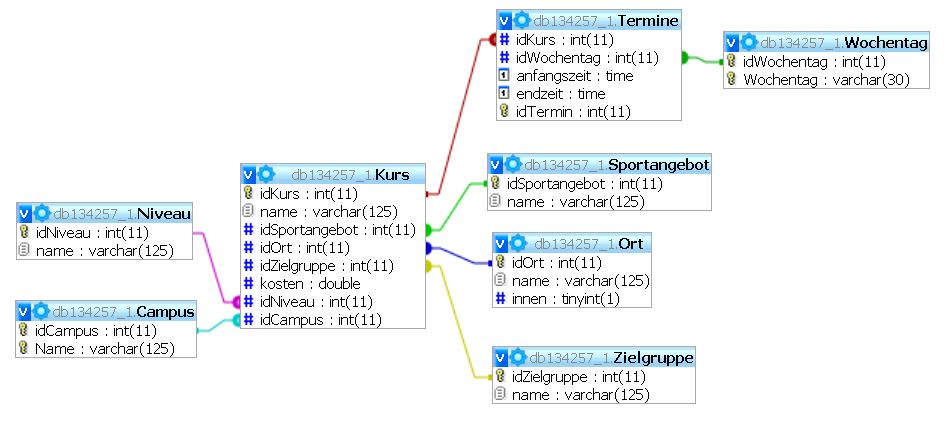
\includegraphics[width=150mm]{images/db_design}
\caption{Datenbank-Design}%
\label{dbd}%
\end{figure}



\section{Ontologie}
Die Ontologie ist das Herzst"uck des Projektes und hat uns einige Probleme bereitet. Zum Erstellen und Bearbeiten der Ontologie im OWL-Format haben wir das Werkzeug Protege eingesetzt.


\section{Programm}
Das Programm wurde mit Java geschreiben und beinhaltet eine Swing-basierte GUI. Funktional ist sie angebunden an eine SQL-Datenbank und eine OWL-Datei.


